\section{Actor Model\label{sec:actor}}
An actor model is a type of concurrency model where the individual workers are the actors. An actor is an independent worker which has its own private state. Actors communicate by sending and receiving asynchronous messages. Each actor processes exactly one message at a time.

\subsection{Understanding the Actor Model Design}
The authors in \cite{8316391} discuss the actor model design by first introducing the actor context. The actor context is the environment where the actors live. It creates actors, tracks them, routes messages to the right actor's mailbox.  The actor is the main unit of work done, in which each actor has a private state, has a mailbox attached, can send messages to other actors and process messages. The mailbox is where the incoming messages for the actor are stored. Processing is not done immediately, but whenever ready, the actor picks up a message from its mailbox and processes it. 
The actor model is illustrated in figure 3. 
\begin{figure}[h]
    \centering
    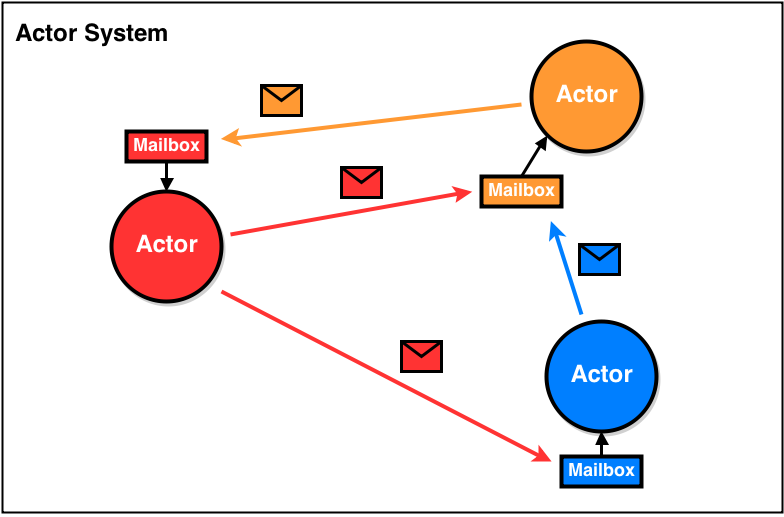
\includegraphics[width=0.7\textwidth]{actor.png}
    \caption{Actors communicating with other actors.}
    \label{fig:actor}
\end{figure}
\subsection{The Actor Model Principle}
The authors in [12] have also discussed regarding certain principles implemented in the actor model.

\begin{table}[h]
    \centering
    \begin{tabular}{|c|c|}
        \hline
        \textbf{Principle} & \textbf{Description} \\
        \hline
        Encapsulation & Each actor has a private internal state, and no actor can view it \\
        \hline
        Internal State & Each actor has its own memory and updates it. \\
        \hline
        Messaging & Actors communicate by sending and receiving \\
        \hline
        Indeterminacy & Messages may arrive in any order \\
        \hline
        
    \end{tabular}
    \caption{Basic Components of the Actor Model}
    \label{tab:actor_model}
\end{table}

\subsection{Data Races and Deadlocks}
A data race occurs when when two or more threads access the same shared memory at the same time, which can corrupt the data. A deadlock occurs when two or more threads are waiting for each other to release a lock and so the system freezes. 

Data races don't occur in the actor model because there is no shared memory between actors, as each actor has its own private state, wherein no other actor can directly read or write that state and every communication happens through messages only. 

Deadlocks don't occur in the actor model as there is asynchronous messaging without any locks. Actors send a message and move on without waiting or blocking. In this no actor is waiting or holding a lock to release a resource.

\subsection{Optimization using Batch Actors}
The authors in \cite{10820772} introduced batch actors to tackle the problem where hundreds of thousands of small tasks all try to synchronize through one actor, which can lead to a communication bottleneck.

Instead of using one main actor executing thousands of tasks, several tasks are grouped under batch actors, and batch actors message the main job actor, which leads to a reduce in contention. 

The experiments had shown that the models were 4x faster than the actor model without batching and resulted in less communication bottlenecks and better scaling.

\subsection{Benchmarks conducted}
The authors in \cite{8892329} conducted various experiments using different libraries implementing the actor model. These were the findings:

\begin{table}[H]
    \centering
    \begin{tabular}{|c|p{5cm}|p{5cm}|}
        \hline
        \textbf{Benchmark} & \textbf{What it Measured} & \textbf{Main Finding} \\
        \hline
        Enqueuing Benchmark & Time taken to push messages into an actor's mailbox. & Scalaz achieved the fastest enqueuing time compared to Akka and Lift. \\
        \hline
        Max Throughput Benchmark & Number of messages processed per second. & Scalaz had the highest throughput performance. \\
        \hline
        Ping Latency Benchmark & Time for a message to travel from one actor to another and back. & Scalaz demonstrated the lowest ping latency. \\
        \hline
        Big Benchmark (Many-to-Many) & Performance under massive actor communication between many actors. & Scalaz scaled better with many actors under stress. \\
        \hline
        Chameneos Benchmark & Handling complex meeting and communication scenarios among actors. & Scalaz outperformed Akka and Lift in this concurrency problem. \\
        \hline
    \end{tabular}
    \caption{Benchmarks conducted and key findings from actor system implementations.}
    \label{tab:benchmarks_conducted}
\end{table}

For pure speed, Scalaz is best for lightweight, fast concurrent systems. But for building robust, distributed systems, Akka is better becauser it offers more built-in tools as well as a good actor lifecycle management and for building complex and fault tolerant systems








